\scanpage{111}
\figure{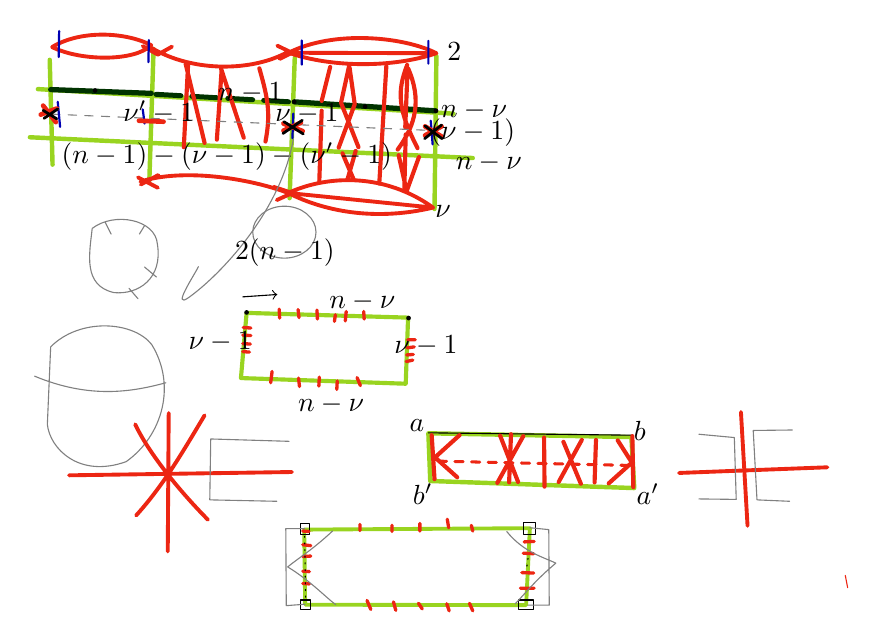
\begin{tikzpicture}[x=.006cm,y=-.006cm,line cap=round,line join=round]
\draw[yellow!60!green,line width=1.6pt] (126,325)--(1006,377) (109,427)--(1047,471) (151,263)--(157,485) (371,240)--(362,519) (670,259)--(659,556) (970,255)--(966,579);
\draw[green!20!black,line width=1.9pt] (153,326)--(366,334) (669,352)--(968,371);
\draw[green!20!black,line width=1.8pt,dash pattern=on 9pt off 4pt] (376,336)--(660,352);
\draw[red!70!brown,line width=1.4pt] (156,236)..controls(217,199)and(312,204)..(366,232)..controls(330,267)and(217,266)..(156,236) (359,233)..controls(445,289)and(575,290)..(654,247) (633,233)--(664,248)--(638,261) (348,234)--(380,252)--(410,235);
\draw[red!70!brown,line width=1.4pt] (657,248)..controls(751,200)and(899,213)..(970,249)..controls(879,280)and(749,280)..(657,248)--(970,249);
\draw[red!70!brown,line width=1.4pt] (343,521)..controls(433,492)and(574,514)..(656,545)..controls(741,506)and(862,503)..(963,576)..controls(849,603)and(741,588)..(656,545)--(963,576) (338,512)--(380,534) (344,527)--(381,507) (625,532)--(665,545)--(632,560);
\draw[red!70!brown,line width=1.5pt] (439,272)--(479,439) (444,274)--(435,448) (514,282)--(562,428) (515,286)--(505,432) (595,281)..controls(614,348)and(619,377)..(608,436) (745,278)--(727,350) (727,371)--(722,520) (786,272)--(768,354)--(805,448) (786,279)--(797,357)--(763,449) (771,461)--(795,517) (799,456)--(782,515) (864,276)--(849,525) (908,274)..controls(887,329)and(887,366)..(930,450) (910,281)..controls(939,347)and(927,400)..(888,453) (909,282)--(904,406) (905,421)--(902,540) (890,465)--(907,541) (933,469)--(907,541);
\draw[gray,dashed] (155,378)--(969,413);
\draw[blue!70!black,line width=.8pt] (171,202)--(170,257) (361,221)--(360,268) (685,222)--(685,273) (953,223)--(953,271) (168,352)--(173,405) (348,368)--(352,398) (667,377)--(665,429) (958,392)--(962,442);
\draw[red!70!brown,line width=1.7pt] (132,379)--(166,366) (137,360)--(164,395) (340,392)--(392,394) (646,398)--(687,414) (646,413)--(683,396) (946,404)--(982,426) (946,423)--(981,404);
\draw[line width=1pt] (137,370)--(166,388) (139,387)--(168,367) (647,394)--(688,420) (645,419)--(686,391) (946,403)--(982,430) (945,430)--(981,401);
\fill (247,328) circle(5);\fill (669,352) circle(5);\fill (819,362) circle(5);\fill (969,371) circle(5);
\node at (1008,246) {$\unsure{2}$};\node at (576,332) {$n-1$};\node at (1050,371) {$n-\nu$};\node at (1047,417) {$(\nu-1)$};\node at (1081,481) {$n-\nu$};\node at (984,585) {$\nu$};\node at (696,377) {$\nu-1$};\node at (382,374) {$\nu'-1$};\node at (526,467) {$(n-1)-(\nu-1)-(\nu'-1)$};
\draw[gray] (241,620)..controls(288,584)and(375,601)..(379,653)..controls(391,726)and(339,761)..(287,756)..controls(221,741)and(235,674)..(241,620) (269,608)--(281,632) (352,614)--(341,632) (352,702)--(377,723) (319,747)--(338,769);
\draw[gray] (667,431)..controls(640,584)and(514,717)..(446,766)..controls(408,793)and(456,721)..(466,701);
\draw[gray] (648,628) ellipse(67 and 55);\node at (649,672) {$2(n-1)$};
\draw[yellow!60!green,line width=1.5pt] (568,799)--(910,809)--(905,949)--(556,937)--cycle;
\fill (568,798) circle(5);\fill (911,810) circle(5);
\draw[->] (560,765)--(633,760);
\draw[red!70!brown,line width=1.2pt] (637,791)--(638,810) (677,792)--(679,809) (717,793)--(718,812) (756,803)--(754,817) (779,796)--(777,816) (816,796)--(817,812) (561,830)--(577,831) (560,846)--(577,847) (560,864)--(576,865) (560,881)--(574,882) (909,856)--(925,856) (908,873)--(923,871) (907,888)--(921,887) (906,902)--(920,899) (622,923)--(619,947) (678,937)--(680,955) (722,935)--(721,954) (760,943)--(759,961) (802,936)--(809,953);
\node at (813,774) {$n-\nu$};\node at (747,993) {$n-\nu$};\node at (512,860) {$\nu-1$};\node at (948,868) {$\nu-1$};
\draw[gray] (153,871)..controls(214,809)and(328,816)..(367,866)..controls(420,952)and(390,1059)..(313,1114)..controls(213,1150)and(151,1086)..(146,1035)--cycle (119,933)..controls(237,982)and(326,966)..(397,947);
\draw[red!70!brown,line width=1.4pt] (192,1143)--(664,1136) (403,1011)--(401,1304) (332,1035)..controls(358,1090)and(416,1166)..(486,1237) (479,1016)..controls(433,1093)and(392,1164)..(334,1228);
\draw[gray] (658,1071)--(492,1066)--(490,1195)--(632,1198);
\draw[yellow!60!green,line width=1.6pt] (953,1054)--(1383,1062)--(1389,1170)--(957,1155)--cycle;
\draw (953,1053)--(1384,1058) (1387,1060)--(1389,1166);
\draw[red!70!brown,line width=1.5pt] (960,1058)--(966,1151) (1019,1058)--(967,1105)--(1014,1147) (1105,1059)--(1143,1157) (1154,1060)--(1099,1159) (1128,1056)--(1124,1158) (1198,1063)--(1199,1167) (1239,1072)--(1276,1161) (1278,1068)--(1229,1157) (1308,1068)--(1305,1158) (1354,1069)--(1384,1116)--(1335,1160) (1385,1060)--(1387,1168);
\draw[red!70!brown,line width=1.1pt,dashed] (974,1113)--(1378,1122);
\node at (929,1038) {$a$};\node at (1401,1048) {$b$};\node at (941,1183) {$b'$};\node at (1418,1183) {$a'$};
\draw[red!70!brown,line width=1.4pt] (1484,1138)--(1798,1126) (1615,1009)--(1629,1250);
\draw[gray] (1526,1056)--(1601,1063)--(1605,1194)--(1526,1193) (1724,1047)--(1641,1048)--(1649,1195)--(1718,1198);
\draw[yellow!60!green,line width=1.4pt] (690,1258)--(1168,1255)--(1160,1418)--(692,1417)--cycle;
\draw (682,1245) rectangle(701,1269) (682,1407) rectangle(704,1427) (1155,1242) rectangle(1179,1268) (1144,1407) rectangle(1176,1427);
\draw[red!70!brown,line width=1.2pt] (808,1247)--(808,1260) (876,1249)--(876,1262) (935,1245)--(935,1261) (993,1236)--(996,1254) (1044,1249)--(1047,1261) (823,1408)--(831,1427) (879,1411)--(884,1429) (932,1414)--(940,1426) (992,1415)--(997,1430) (1040,1414)--(1047,1430) (687,1261)--(700,1262) (687,1290)--(704,1292) (687,1315)--(704,1314) (687,1346)--(701,1347) (687,1372)--(701,1373) (1156,1284)--(1177,1283) (1154,1308)--(1176,1309) (1151,1349)--(1176,1350) (1148,1382)--(1177,1382);
\draw[dotted] (691,1272)--(693,1404) (1164,1319)--(1161,1340);
\draw[gray] (691,1256)--(651,1256)--(652,1419)--(692,1416) (1168,1254)--(1208,1258)--(1209,1418)--(1164,1418) (750,1261)..controls(706,1302)and(678,1318)..(655,1337)..controls(704,1367)and(735,1401)..(757,1417) (1119,1262)..controls(1154,1305)and(1193,1315)..(1223,1329)..controls(1181,1364)and(1159,1392)..(1137,1415);
\draw[red!70!brown] (1836,1355)--(1841,1381);
\end{tikzpicture}}
\[
\deleted{n-\nu-\nu'+1}\qquad n-1\qquad\deleted{n-1}
\]
\[
n-(\nu+\nu'-1)=(n-1)\unsure{-|\leftarrow}(\nu-1)-(\nu'-1)
\qquad n-\nu-(\nu'-1)\qquad n
\]
\figure{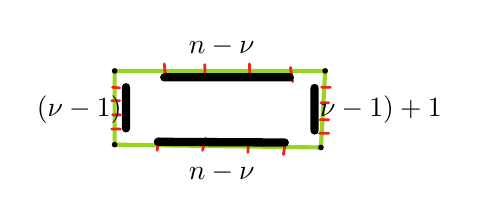
\begin{tikzpicture}[x=.009cm,y=-.009cm,line cap=round]
\draw[yellow!60!green,line width=1.5pt] (0,0)--(297,0)--(291,108)--(0,104)--cycle;
\fill (0,0) circle(4);\fill (297,0) circle(4);\fill (291,108) circle(4);\fill (0,104) circle(4);
\draw[red!70!brown,line width=1pt] (70,-10)--(72,10) (127,-9)--(128,11) (190,-10)--(191,10) (248,-5)--(251,15) (62,95)--(60,112) (128,95)--(124,112) (189,97)--(188,115) (241,101)--(238,118) (-3,23)--(7,24) (-4,42)--(7,42) (-3,62)--(8,62) (-4,82)--(8,82) (292,23)--(304,23) (291,45)--(302,45) (290,69)--(302,69) (289,88)--(302,88);
\draw[line width=3pt] (70,9)--(247,9) (61,100)--(240,101) (16,23)--(16,81) (282,24)--(282,84);
\node at (151,-35) {$n-\nu$};\node at (151,143) {$n-\nu$};\node at (-50,54) {$(\nu-1)$};\node at (368,55) {$(\nu-1)+1$};
\end{tikzpicture}}
\figure{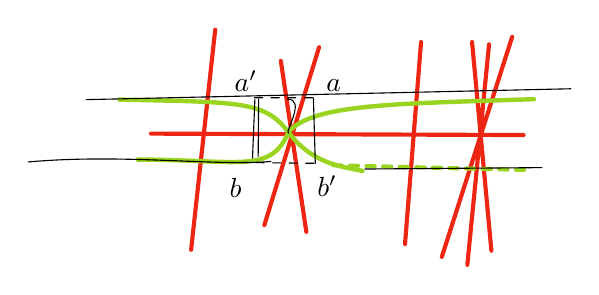
\begin{tikzpicture}[x=.006cm,y=-.006cm,line cap=round,line join=round]
\draw[red!70!brown,line width=1.5pt] (1268,759)--(2057,762) (1404,539)--(1353,1005) (1543,605)--(1597,967) (1624,576)--(1508,953) (1840,565)--(1806,993) (1948,565)--(1989,1007) (1984,570)--(1938,1037) (2033,554)--(1884,1020);
\draw[yellow!60!green,line width=1.6pt] (1201,687)..controls(1461,692)and(1510,691)..(1559,756)..controls(1611,825)and(1676,829)..(1716,838);
\draw[yellow!60!green,line width=1.6pt] (1240,814)..controls(1455,814)and(1522,845)..(1559,756)..controls(1610,695)and(1791,696)..(2079,686);
\draw[yellow!60!green,line width=1.5pt,dashed] (1654,826)--(2064,836);
\draw (1131,687)--(2157,664) (1008,819)..controls(1210,801)and(1398,828)..(1522,818) (1721,834)--(2096,831);
\draw[dashed] (1487,683)--(1612,683) (1455,820)--(1625,822);
\draw (1488,687)--(1483,811) (1496,686)--(1495,807) (1612,683)--(1616,822) (1557,686)..controls(1597,686)and(1551,756)..(1559,758);
\node at (1469,647) {$a'$};\node at (1655,657) {$a$};\node at (1447,875) {$b$};\node at (1641,871) {$b'$};
\end{tikzpicture}}
\[
n-\nu\qquad n-\nu-(\nu'-1)
\]
\[
\begin{array}{ccc}
&n-\nu'&\\&n-\nu'&\\\nu&n-\nu'&\nu\\&n-1&
\end{array}
\qquad
\begin{array}{l}
n-\nu\\
2n-\deleted{\unsure{2}}\nu-\deleted{\unsure{2}}\nu'+2\\
2n-\underbrace{(\nu+\nu'-2)}_{\unsure{\varepsilon|\xi}\geq2}
\end{array}
\]
\[
2n-2(\nu+\nu'-1)\qquad
2n-(\nu+\nu'-1)\qquad
\deleted{2n}\quad 2n-(\nu+\nu'-1)
\]

\figure{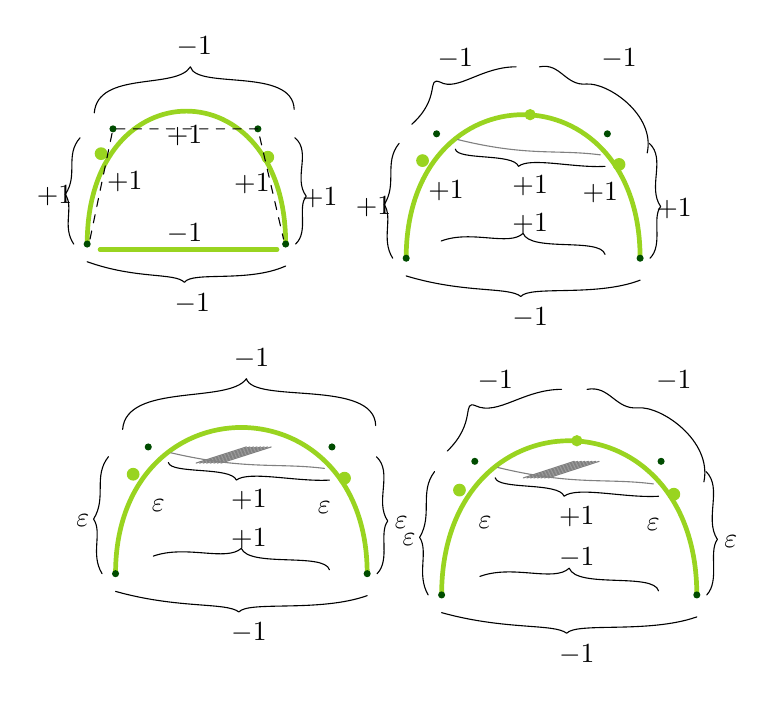
\begin{tikzpicture}[x=.009cm,y=-.009cm,line cap=round,line join=round]
\begin{scope}[shift={(0,0)} ]
\draw[yellow!60!green,line width=1.7pt] (0,250) .. controls (0,0) and (280,0) .. (280,250);
\fill[green!30!black] (0,250) circle(5);
\fill[green!30!black] (36.4,87.5) circle(5);
\fill[green!30!black] (240.79999999999998,87.5) circle(5);
\fill[green!30!black] (280,250) circle(5);
\fill[yellow!60!green] (19.6,122.5) circle(9);
\fill[yellow!60!green] (254.8,127.5) circle(9);
\draw[yellow!60!green,line width=1.6pt] (18,258)--(268,258);
\draw[dashed] (4,243)--(36.4,87.5)--(240.79999999999998,87.5)--(277,243);
\draw (10,65.0) .. controls(15,5.0)and(126.0,32.5)..(145.6,0) .. controls(154.0,32.5)and(290,0)..(292,60.0);
\node at (151.20000000000002,-28) {$-1$};
\draw (0,275) .. controls(70.0,300)and(123.2,290)..(137.2,304) .. controls(148.4,288)and(226.8,305)..(280,281);
\node at (148.4,334) {$-1$};
\draw (-10,100.0) .. controls(-32,125.0)and(-12,152.5)..(-31,180.0) .. controls(-18,197.5)and(-36,225.0)..(-19,250);
\node at (-46,182.5) {$+1$};
\draw (293,100.0) .. controls(317,120.0)and(290,157.5)..(309,182.5) .. controls(296,197.5)and(313,232.5)..(294,250);
\node at (328,185.0) {$+1$};
\node at (137.2,97.5) {$+1$};\node at (53.2,162.5) {$+1$};\node at (232.39999999999998,165.0) {$+1$};\node at (137.2,235.0) {$-1$};
\end{scope}
\begin{scope}[shift={(450,0)} ]
\draw[yellow!60!green,line width=1.7pt] (0,270) .. controls (0,0) and (330,0) .. (330,270);
\fill[green!30!black] (0,270) circle(5);
\fill[green!30!black] (42.9,94.5) circle(5);
\fill[green!30!black] (283.8,94.5) circle(5);
\fill[green!30!black] (330,270) circle(5);
\fill[yellow!60!green] (23.1,132.3) circle(9);
\fill[yellow!60!green] (300.3,137.7) circle(9);
\fill[yellow!60!green] (174.9,67.5) circle(8);
\draw[gray] (72.6,102.6)..controls(171.6,126.89999999999999)and(211.20000000000002,116.1)..(273.9,124.2);
\draw (8,81.0) .. controls(50,43.2)and(28,13.5)..(48,21.6) .. controls(72.6,35.1)and(105.60000000000001,0)..(155.1,0);
\node at (69.3,-12) {$-1$};
\draw (188.1,0) .. controls(217.8,-6)and(224.4,27.0)..(254.1,24.3) .. controls(283.8,21.6)and(352,67.5)..(340,121.5);
\node at (300.3,-12) {$-1$};
\draw (0,295) .. controls(82.5,320)and(145.2,310)..(161.7,324) .. controls(174.9,308)and(267.3,325)..(330,301);
\node at (174.9,354) {$-1$};
\draw (-10,108.0) .. controls(-32,135.0)and(-12,164.7)..(-31,194.4) .. controls(-18,213.3)and(-36,243.0)..(-19,270);
\node at (-46,197.1) {$+1$};
\draw (343,108.0) .. controls(367,129.6)and(340,170.1)..(359,197.1) .. controls(346,213.3)and(363,251.10000000000002)..(344,270);
\node at (378,199.8) {$+1$};
\draw (69.3,116.1) .. controls(72.6,132.3)and(151.8,121.5)..(158.4,140.4) .. controls(174.9,126.89999999999999)and(237.6,143.1)..(280.5,140.4);
\node at (174.9,167.4) {$+1$};
\draw (49.5,245.70000000000002) .. controls(92.4,229.5)and(145.2,253.79999999999998)..(165.0,234.9) .. controls(174.9,261.9)and(273.9,240.3)..(280.5,264.6);
\node at (174.9,221.39999999999998) {$+1$};
\node at (56.1,175.5) {$+1$};
\node at (273.9,178.20000000000002) {$+1$};
\end{scope}
\begin{scope}[shift={(40,440)} ]
\draw[yellow!60!green,line width=1.7pt] (0,275) .. controls (0,0) and (355,0) .. (355,275);
\fill[green!30!black] (0,275) circle(5);
\fill[green!30!black] (46.15,96.25) circle(5);
\fill[green!30!black] (305.3,96.25) circle(5);
\fill[green!30!black] (355,275) circle(5);
\fill[yellow!60!green] (24.85,134.75) circle(9);
\fill[yellow!60!green] (323.05,140.25) circle(9);
\draw[gray] (78.1,104.5)..controls(184.6,129.25)and(227.20000000000002,118.25)..(294.65,126.5);
\draw (10,71.5) .. controls(15,5.5)and(159.75,35.75)..(184.6,0) .. controls(195.25000000000003,35.75)and(365,0)..(367,66.0);
\node at (191.70000000000002,-28) {$-1$};
\draw (0,300) .. controls(88.75,325)and(156.2,315)..(173.95,329) .. controls(188.15,313)and(287.55,330)..(355,306);
\node at (188.15,359) {$-1$};
\draw (-10,110.0) .. controls(-32,137.5)and(-12,167.75)..(-31,198.0) .. controls(-18,217.25)and(-36,247.5)..(-19,275);
\node at (-46,200.75) {$\varepsilon$};
\draw (368,110.0) .. controls(392,132.0)and(365,173.25)..(384,200.75) .. controls(371,217.25)and(388,255.75)..(369,275);
\node at (403,203.5) {$\varepsilon$};
\draw (74.55,118.25) .. controls(78.1,134.75)and(163.3,123.75)..(170.4,143.0) .. controls(188.15,129.25)and(255.6,145.75)..(301.75,143.0);
\node at (188.15,170.5) {$+1$};
\draw (53.25,250.25) .. controls(99.4,233.75)and(156.2,258.5)..(177.5,239.25) .. controls(188.15,266.75)and(294.65,244.75)..(301.75,269.5);
\node at (188.15,225.5) {$+1$};
\node at (60.35,178.75) {$\varepsilon$};
\node at (294.65,181.5) {$\varepsilon$};
\draw[gray] (113.60000000000001,119.0)--(184.6,96.25);
\draw[gray] (118.60000000000001,119.0)--(189.6,96.25);
\draw[gray] (123.60000000000001,119.0)--(194.6,96.25);
\draw[gray] (128.60000000000002,119.0)--(199.6,96.25);
\draw[gray] (133.60000000000002,119.0)--(204.6,96.25);
\draw[gray] (138.60000000000002,119.0)--(209.6,96.25);
\draw[gray] (143.60000000000002,119.0)--(214.6,96.25);
\draw[gray] (148.60000000000002,119.0)--(219.6,96.25);
\end{scope}
\begin{scope}[shift={(500,455)} ]
\draw[yellow!60!green,line width=1.7pt] (0,290) .. controls (0,0) and (360,0) .. (360,290);
\fill[green!30!black] (0,290) circle(5);
\fill[green!30!black] (46.800000000000004,101.5) circle(5);
\fill[green!30!black] (309.6,101.5) circle(5);
\fill[green!30!black] (360,290) circle(5);
\fill[yellow!60!green] (25.200000000000003,142.1) circle(9);
\fill[yellow!60!green] (327.6,147.9) circle(9);
\fill[yellow!60!green] (190.8,72.5) circle(8);
\draw[gray] (79.2,110.2)..controls(187.20000000000002,136.29999999999998)and(230.4,124.7)..(298.8,133.4);
\draw (8,87.0) .. controls(50,46.4)and(28,14.5)..(48,23.2) .. controls(79.2,37.7)and(115.2,0)..(169.2,0);
\node at (75.6,-12) {$-1$};
\draw (205.2,0) .. controls(237.60000000000002,-6)and(244.8,29.0)..(277.2,26.099999999999998) .. controls(309.6,23.2)and(382,72.5)..(370,130.5);
\node at (327.6,-12) {$-1$};
\draw (0,315) .. controls(90.0,340)and(158.4,330)..(176.4,344) .. controls(190.8,328)and(291.6,345)..(360,321);
\node at (190.8,374) {$-1$};
\draw (-10,116.0) .. controls(-32,145.0)and(-12,176.9)..(-31,208.79999999999998) .. controls(-18,229.10000000000002)and(-36,261.0)..(-19,290);
\node at (-46,211.7) {$\varepsilon$};
\draw (373,116.0) .. controls(397,139.2)and(370,182.7)..(389,211.7) .. controls(376,229.10000000000002)and(393,269.7)..(374,290);
\node at (408,214.6) {$\varepsilon$};
\draw (75.6,124.7) .. controls(79.2,142.1)and(165.6,130.5)..(172.79999999999998,150.8) .. controls(190.8,136.29999999999998)and(259.2,153.70000000000002)..(306.0,150.8);
\node at (190.8,179.8) {$+1$};
\draw (54.0,263.90000000000003) .. controls(100.80000000000001,246.5)and(158.4,272.59999999999997)..(180.0,252.3) .. controls(190.8,281.3)and(298.8,258.1)..(306.0,284.2);
\node at (190.8,237.79999999999998) {$-1$};
\node at (61.2,188.5) {$\varepsilon$};
\node at (298.8,191.4) {$\varepsilon$};
\draw[gray] (115.2,125.0)--(187.20000000000002,101.5);
\draw[gray] (120.2,125.0)--(192.20000000000002,101.5);
\draw[gray] (125.2,125.0)--(197.20000000000002,101.5);
\draw[gray] (130.2,125.0)--(202.20000000000002,101.5);
\draw[gray] (135.2,125.0)--(207.20000000000002,101.5);
\draw[gray] (140.2,125.0)--(212.20000000000002,101.5);
\draw[gray] (145.2,125.0)--(217.20000000000002,101.5);
\draw[gray] (150.2,125.0)--(222.20000000000002,101.5);
\end{scope}
\end{tikzpicture}}
\[
\varepsilon=\begin{cases}
+1&\text{si la \unsure{face} spéciale est du}\\
&\text{type sommet (ultra \unsure{spécial})}\\
-1&\text{sinon}
\end{cases}
\]
Comment trouver le \unsure{calcul|valeur} de $\varepsilon$ ?
\margin{\begin{tabular}{l}
\texttt{//*JOB=CRAY2,ACCT=\unsure{*********},ALL=NO,MSGL=N}\qquad\texttt{J0296CNU}\\
\texttt{// JOB MSGLEVEL=(1,1),MSGCLASS=A}\\
\texttt{// EXEC PGM=IEFBR14}
\end{tabular}}
\margin{110}
